%\VignetteIndexEntry{testerccdashboard examples}

\documentclass{article}
\usepackage{fullpage}
\usepackage{Sweave}
\begin{document}
\Sconcordance{concordance:erccdashboardVignette.tex:erccdashboardVignette.Rnw:%
1 4 1 1 0 8 1 1 6 17 1 1 2 4 0 1 2 1 3 5 0 1 2 2 1 1 %
2 12 0 1 1 6 0 1 2 14 1 1 2 1 0 1 1 3 0 1 2 4 1 1 2 4 %
0 1 2 14 1 1 2 1 0 4 1 3 0 1 2 2 1 1 2 4 0 1 2 5 1 1 %
3 12 0 2 2 21 0 1 2 8 1 1 2 31 0 1 2 9 1 1 3 13 0 1 2 %
5 1 1 2 11 0 1 2 4 1 1 2 10 0 1 2 4 1 1 2 10 0 1 2 4 %
1 1 3 17 0 1 2 5 1 1 2 27 0 2 2 5 0 1 2 1 1 1 2 5 0 1 %
2 1 1 1 2 5 0 1 2 3 1 1 2 4 0 1 2 2 1 1 2 4 0 1 2 5 1}



\DefineVerbatimEnvironment{Sinput}{Verbatim} {xleftmargin=1em}
\DefineVerbatimEnvironment{Soutput}{Verbatim}{xleftmargin=1em}
\DefineVerbatimEnvironment{Scode}{Verbatim}{xleftmargin=1em}
\fvset{listparameters={\setlength{\topsep}{0pt}}}
\renewenvironment{Schunk}{\vspace{\topsep}}{\vspace{\topsep}}
    
\title{{\tt testerccdashboard} Package Example}
\author{Sarah A. Munro}
\maketitle

\begin{center}
\Large
{\tt erccdashboard} Package Vignette
\normalsize
\end{center}
This vignette describes the use of the erccdashboard R package to analyze 
External RNA Control Consortium (ERCC) spike-in control ratio mixtures in gene
expression experiments. Two types of data from the SEQC/MAQC III project were analyzed.
\begin{enumerate}
  \item Rat toxicogenomics treatment and control samples for different drug 
  treatments
  \item Human reference RNA samples from the MAQC I project, Universal Human 
  Reference RNA (UHRR) and Human Brain Reference RNA (HBRR)
\end{enumerate}

\section{Rat Toxicogenomics Example: MET treatment}
\subsection{Define input data and parameters}

Load the testerccdashboard package. 
\begin{Schunk}
\begin{Sinput}
> library( "testerccdashboard" )
\end{Sinput}
\end{Schunk}
Load the Rat Toxicogenomics Data set.
\begin{Schunk}
\begin{Sinput}
> load(file = system.file("data/SEQC.RatTox.Example.RData", 
                          package = "testerccdashboard"))
\end{Sinput}
\end{Schunk}
The R workspace should now contain 5 count tables and for each count table a 
corresponding total reads vector.
Take a look at the data for the MET experiment.
\begin{Schunk}
\begin{Sinput}
> head(COH.RatTox.ILM.MET.CTL.countTable)
\end{Sinput}
\begin{Soutput}
     Feature MET_1 MET_2 MET_3 CTL_1 CTL_2 CTL_3
1 ERCC-00002 16629 18798 26568 36600 45436 25163
2 ERCC-00003  1347  1565  1983  3048  3447  2195
3 ERCC-00004  4569  5570  6755  1240  1484   902
4 ERCC-00009   811   869  1123   909  1073   537
5 ERCC-00013     3     1     2     1     5     1
6 ERCC-00019    24    32    43     5    13     4
\end{Soutput}
\begin{Sinput}
> COH.RatTox.ILM.MET.CTL.totalReads
\end{Sinput}
\begin{Soutput}
[1] 41423502 46016148 44320280 38400362 47511484 33910098
\end{Soutput}
\end{Schunk}
The first column of the count table, Feature, contains unique names for all
the transcripts that were quantified in this experiment. The remaining columns
represent replicates of the pair of samples, in this count table 
the control sample is labeled CTL and the treatment sample is labeled MET. An underscore is included to separate the sample names from the replicate numbers during analysis. This naming convention Sample\textunderscore{}Rep is needed for the columns of any input count table.

The total reads vectors will be used for library size normalization of the count
tables. Total reads can either represent the total number of reads in FASTQ 
files or total mapped reads. In the examples provided with this package FASTQ 
file total reads are used.

For our analysis of the MET-CTL experiment start by assigning the MET-CTL data to the input data variables countTable and totalReads.
\begin{Schunk}
\begin{Sinput}
> countTable <- COH.RatTox.ILM.MET.CTL.countTable
> totalReads <- COH.RatTox.ILM.MET.CTL.totalReads
\end{Sinput}
\end{Schunk}
In addition to countTable and totalReads, there are 7 additional variables that must be defined by the user. First the filename prefix for results files, filenameRoot, needs to be defined. Here we choose to use the lab abbreviation COH and the platform abbreviation ILM as our identifiers, but this is flexible for the user.
\begin{Schunk}
\begin{Sinput}
> filenameRoot = "COH.ILM"
\end{Sinput}
\end{Schunk}
Next, 5 parameters associated with the ERCC control ratio mixtures need to be defined, sample1Name, sample2Name, ERCCdilution, spikeVol, and totalRNAmass.

The sample spiked with ERCC Mix 1 is sample1Name and the sample spiked with ERCC Mix 2 is sample2Name. In this experiment sample1Name = MET and sample2Name = CTL. For a more robust experimental design the reverse spike-in design could also be produced using additional replicates of the treatment and control samples. ERCC Mix 2 would be spiked into MET samples and ERCC Mix 1 would be spiked into CTL control replicates. 

The dilution factor of the pure Ambion ERCC mixes prior to spiking is ERCCdilution. If no dilution was performed then ERCCdilution should be 1. The amount of diluted ERCC mix spiked into the total RNA sample is spikeVol (units are $\mu$L). The mass of total RNA spiked with the diluted ERCC mix is totalRNAmass (units are $\mu$g )
\begin{Schunk}
\begin{Sinput}
> sample1Name = "MET"
> sample2Name = "CTL"
> ERCCdilution = 1/100
> spikeVol = 1
> totalRNAmass = 0.500
\end{Sinput}
\end{Schunk}
The final required input parameter, choseFDR, is the False Discovery Rate (FDR) for differential expression testing. A typical choice would be 0.05 (5\% FDR), for the rat data a more liberal FDR was used, choseFDR = 0.1.
\begin{Schunk}
\begin{Sinput}
> choseFDR = 0.1
\end{Sinput}
\end{Schunk}
In addition to the required input variables the user can also choose whether to print the results directly to a PDF file (the default is TRUE) with the variable printPDF.
\subsection{Use initDat function to create expDat}
The expDat list is created with the initDat function:
\begin{Schunk}
\begin{Sinput}
> expDat <- initDat(countTable, totalReads, filenameRoot, sample1Name,
                    sample2Name, ERCCdilution, spikeVol, totalRNAmass, choseFDR,
                    printPDF = F)
\end{Sinput}
\begin{Soutput}
[1] "COH.ILM.MET.CTL"
[1] "Library sizes:"
[1] 41.42350 46.01615 44.32028 38.40036 47.51148 33.91010
[1] "Using total sequencing reads mean library size = "
[1] 41.93031
\end{Soutput}
\end{Schunk}
Look at the structure of expDat
\begin{Schunk}
\begin{Sinput}
> summary(expDat)
\end{Sinput}
\begin{Soutput}
                Length Class      Mode      
sampleInfo      17     -none-     list      
totalReads       6     -none-     numeric   
Transcripts      7     data.frame list      
designMat        3     data.frame list      
sampleNames      2     -none-     character 
idCols           6     data.frame list      
totalReads       6     -none-     numeric   
expressDat       7     data.frame list      
libeSize         6     -none-     numeric   
ERCCxlabelIndiv  1     -none-     expression
ERCCxlabelAve    1     -none-     expression
spikeFraction    1     -none-     numeric   
mnLibeFactor     1     -none-     numeric   
sampleLibeSums   6     -none-     numeric   
\end{Soutput}
\end{Schunk}
Estimate r$_m$ for the sample pair using a negative binomial glm
\begin{center}
\begin{Schunk}
\begin{Sinput}
> expDat <- est_r_m(expDat, cnt = expDat$Transcripts, printPlot = T)
\end{Sinput}
\begin{Soutput}
Check for sample mRNA fraction differences(r_m)...

log.offset
17.53936 17.6445 17.60695 17.46358 17.67648 17.33922 

Number of ERCC Controls Used in r_m estimate
63 
Outlier ERCCs for GLM r_m Estimate:
None 
 GLM log(r_m) estimate:
-0.0472291GLM log(r_m) estimate standard deviation:
0.02061546 
63 
 GLM r_m estimate:
0.9538688 
upper limit
0.9599503 
lower limit
0.9478259 
\end{Soutput}
\end{Schunk}
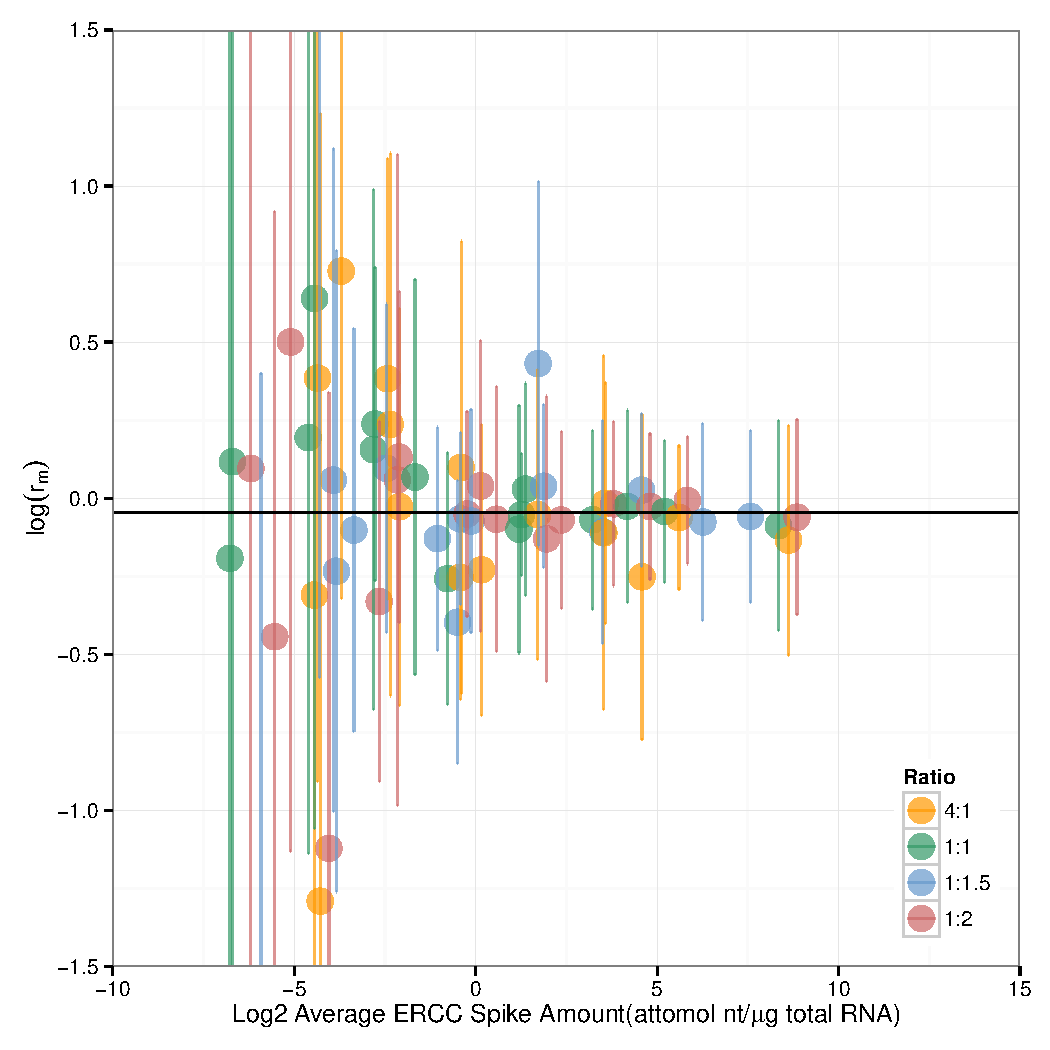
\includegraphics{erccdashboardVignette-est_r_m}
\end{center}
Test for differential expression with geneExprTest
\begin{center}
\begin{Schunk}
\begin{Sinput}
> expDat <- geneExprTest(expDat, cnt = expDat$Transcripts,
                         designMat = expDat$designMat )
\end{Sinput}
\begin{Soutput}
 Differential expression test results exist, will use   
 existing results for analysis. No dispersion plots will
 be produced. Delete COH.ILM.MET.CTL.quasiSeq.res.csv if  
 you want to repeat differential expression testing.    

Threshold P-value
0.006679804 
\end{Soutput}
\end{Schunk}
\end{center}
Generate ROC curves for the selected differential ratios
\begin{center}
\begin{Schunk}
\begin{Sinput}
> erccROC.res = erccROC(expDat)
\end{Sinput}
\begin{Soutput}
  Ratio   AUC Measured Spiked
1   4:1 1.000       16     23
2 1:1.5 0.950       16     23
3   1:2 0.967       16     23
\end{Soutput}
\end{Schunk}
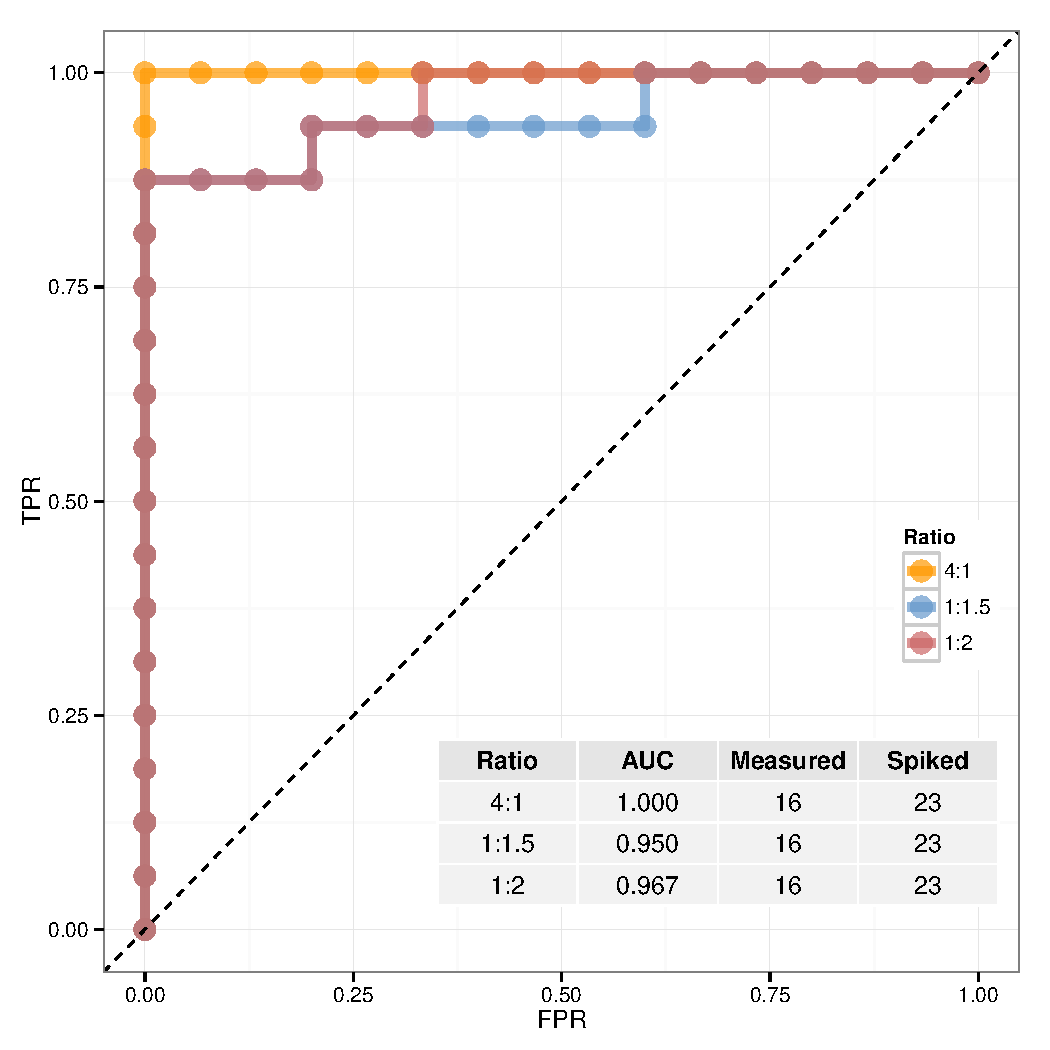
\includegraphics{erccdashboardVignette-erccROC}
\end{center}
Find LODR estimates using the ERCC data p-values.
\begin{center}
\begin{Schunk}
\begin{Sinput}
> lodr.ERCC = estLODR(expDat,kind = "ERCC", prob=0.9)
\end{Sinput}
\begin{Soutput}
  Ratio LODR Estimate 90% CI Lower Bound 90% CI Upper Bound
1   4:1            26                 19                 31
3 1:1.5           Inf               <NA>               <NA>
4   1:2           240                120                340
\end{Soutput}
\end{Schunk}
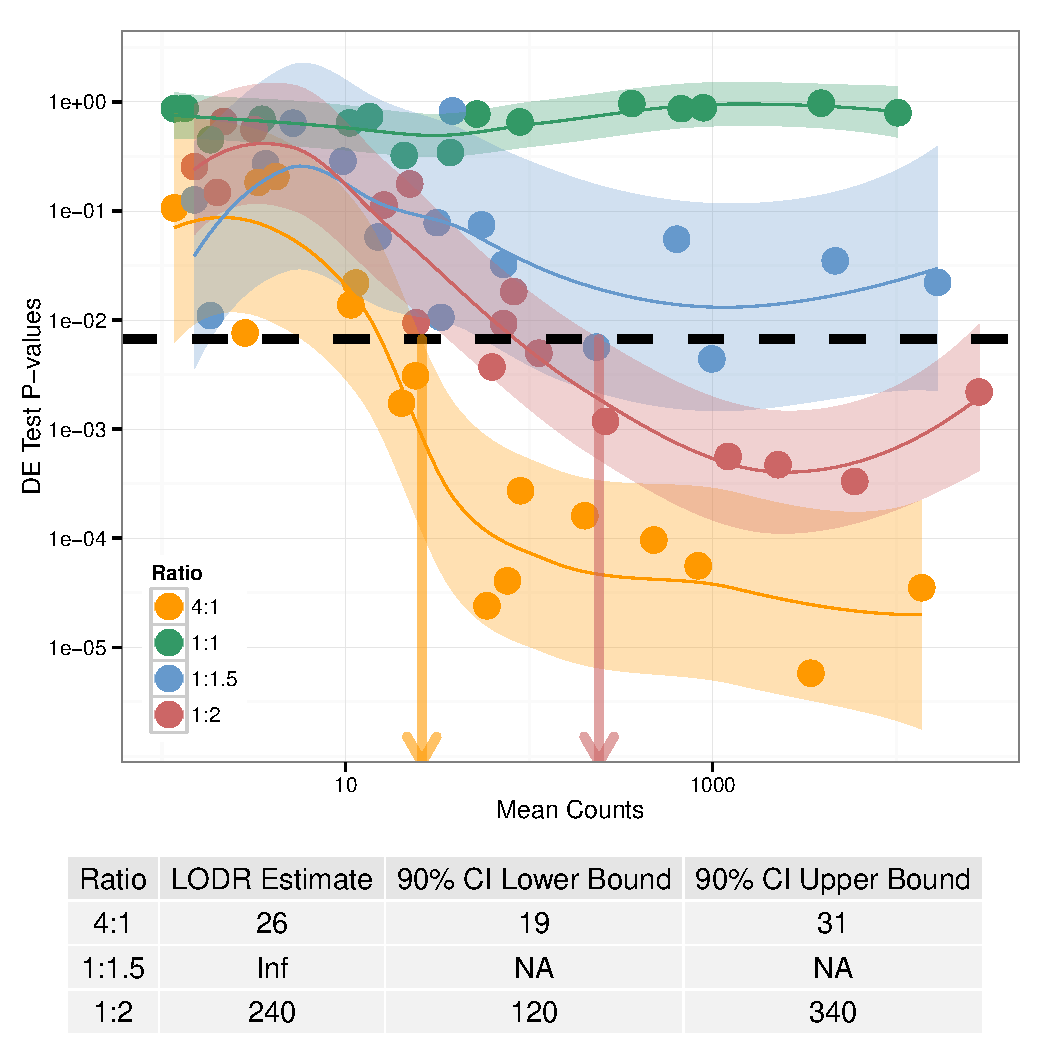
\includegraphics{erccdashboardVignette-estLODRERCC}
\end{center}
One can also obtain LODR estimates using p-values simulated from endogenous transcripts
\begin{center}
\begin{Schunk}
\begin{Sinput}
> lodr.Sim = estLODR(expDat, kind = "Sim", prob = 0.9)  
\end{Sinput}
\begin{Soutput}
  Ratio LODR Estimate 90% CI Lower Bound 90% CI Upper Bound
1   4:1            33                 23                 54
3 1:1.5           Inf               <NA>               <NA>
4   1:2           Inf               <NA>               <NA>
\end{Soutput}
\end{Schunk}
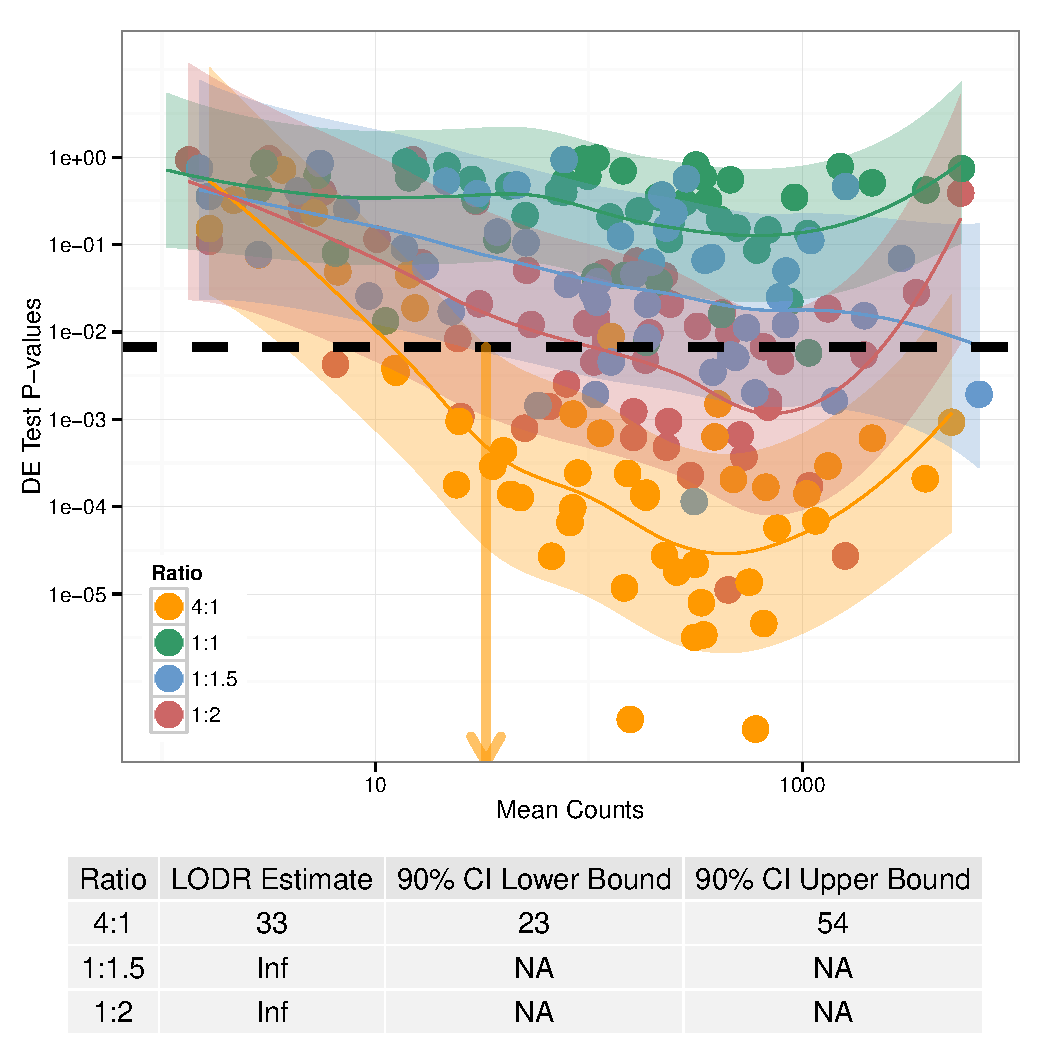
\includegraphics{erccdashboardVignette-estLODRSim}
\end{center}
\subsection{Use dynRangePlot function to evaluate dynamic range data}
Evaluate the dynamic range of the experiment using the ERCC controls.
\begin{center}
\begin{Schunk}
\begin{Sinput}
> dynRangeDat = dynRangePlot(expDat, expressDat = expDat$expressDat,
                             designMat = expDat$designMat, noErrorBars = F)
\end{Sinput}
\begin{Soutput}
[1] "Number of ERCCs in Mix 1 dyn range:"
[1] 63
[1] "Number of ERCCs in Mix 2 dyn range:"
[1] 63
These ERCCs were not included in the signal-abundance plot,
because not enough non-zero replicate measurements of these 
controls were obtained for both samples:
 [1] "ERCC-00058" "ERCC-00067" "ERCC-00077" "ERCC-00168"
 [5] "ERCC-00028" "ERCC-00033" "ERCC-00040" "ERCC-00109"
 [9] "ERCC-00154" "ERCC-00158"
\end{Soutput}
\end{Schunk}
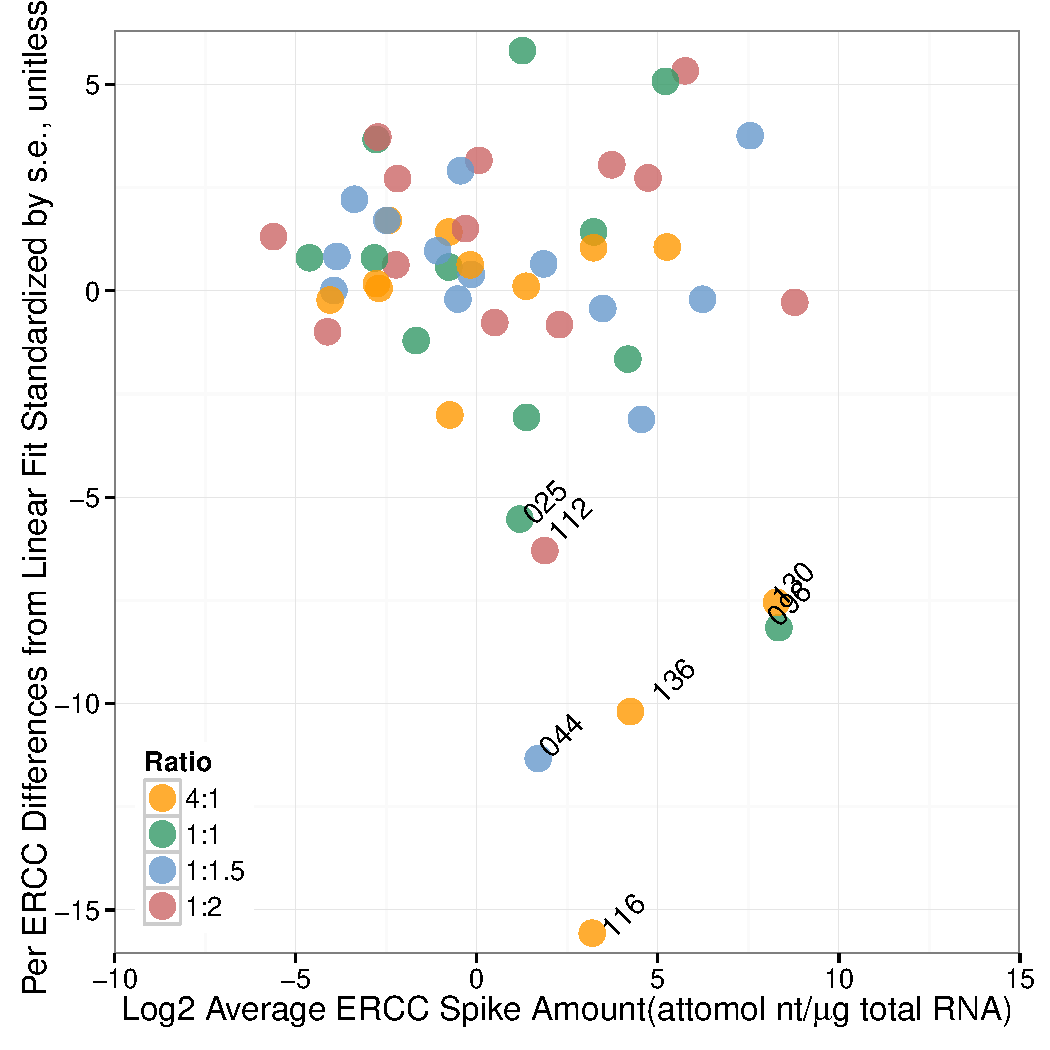
\includegraphics{erccdashboardVignette-dynRangeDat}
\end{center}
\subsection{Use LODR estimates to annote Ratio-Abundance Plot}
Get LODR annotations for adding to plots and then annotate the dynamic range plot with LODR estimate information.
\begin{center}
\begin{Schunk}
\begin{Sinput}
> LODR.annot.ERCC <- printLODRres(expDat, dynRangeDat,
                                  lodr.res = lodr.ERCC)
\end{Sinput}
\begin{Soutput}
   Fold Ratio Count Log2Count_normalized  Log2Conc
1   4:1   4:1    26            -0.689482 -1.106341
2   1:1   1:1    NA                   NA        NA
3 1:1.5 1:1.5   Inf                  Inf       Inf
4   1:2   1:2   240             2.516969  2.172251
\end{Soutput}
\begin{Sinput}
> dynRangePlotLODR(dynRangeRes = dynRangeDat$dynRangePlotRes,
                   LODR.annot.ERCC = LODR.annot.ERCC)
\end{Sinput}
\end{Schunk}
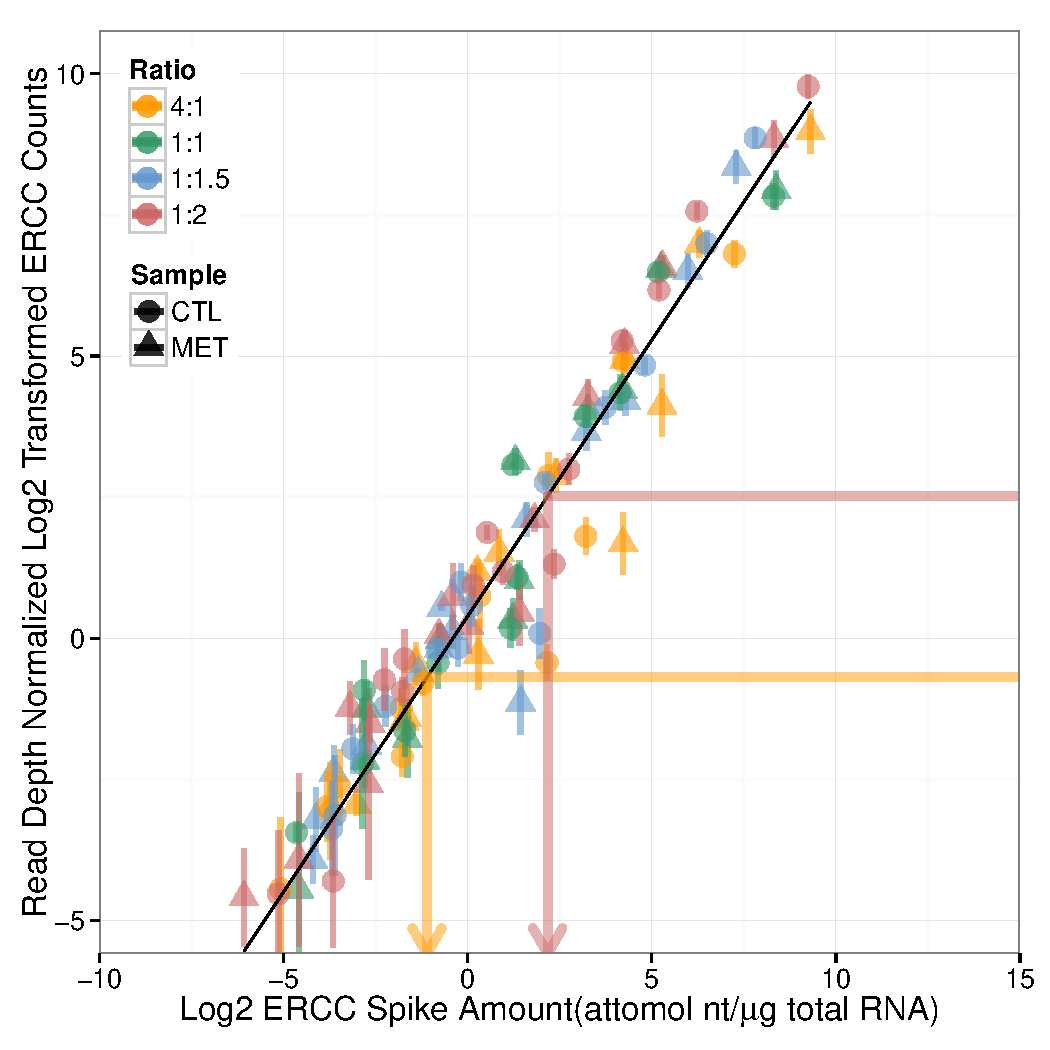
\includegraphics{erccdashboardVignette-dynRangeLODRAnnot}
\end{center}
Generate MA plots of erccs coded by concentrations from LODR
\begin{center}
\begin{Schunk}
\begin{Sinput}
> maPlotAB = maConcPlot(expDat, LODR.annot.ERCC, alphaPoint = 0.8, r_mAdjust = T, 
                        replicate = T)
\end{Sinput}
\begin{Soutput}
[1] "LODR estimates will be used to code ratio-abundance plot"
[1] "These ERCCs were not included in the ratio-abundance plot,  because not enough non-zero replicate measurements of these  controls were obtained for both samples:"
 [1] "ERCC-00028" "ERCC-00033" "ERCC-00040" "ERCC-00058"
 [5] "ERCC-00067" "ERCC-00077" "ERCC-00109" "ERCC-00154"
 [9] "ERCC-00158" "ERCC-00168"
[1] "Global Ratio SD for this sample pair is:"
[1] 0.7785041
                     Estimate Std. Error   t value
Minimum SD Estimate 0.4787852 0.03264151 14.667986
Maximum SD Estimate 1.6195817 0.20936506  7.735683
Lambda              0.4123437 0.05767326  7.149652
                        Pr(>|t|)
Minimum SD Estimate 4.049430e-20
Maximum SD Estimate 3.770026e-10
Lambda              3.158191e-09
[1] "Printing MA plot with LODR coding"
\end{Soutput}
\end{Schunk}
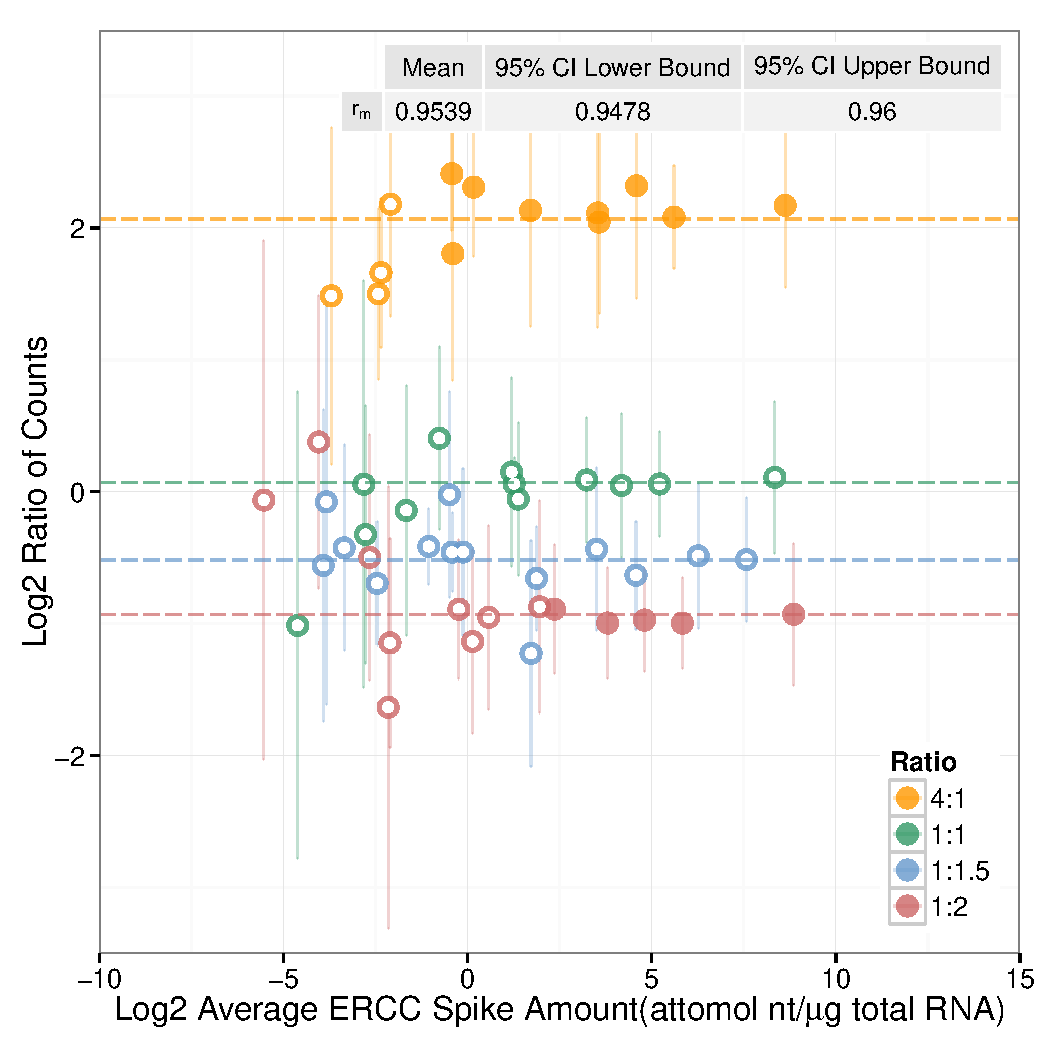
\includegraphics{erccdashboardVignette-maConcPlot}
\end{center}
If you wish, save your results to an Rdata file that can be reused.
\begin{Schunk}
\begin{Sinput}
> saveResults(expDat, erccROC.res, maPlotAB, lodr.ERCC)
\end{Sinput}
\end{Schunk}
\end{document}
